% don't remove the folling lines, and edit the defintion of \main if needed
\documentclass[../report.tex]{subfiles}
\providecommand{\main}{..}
\IfEq{\jobname}{\currfilebase}{\AtEndDocument{\biblio}}{}
% until here
%\usepackage{cite}

\begin{document}
\section{Axions and ALPs}
This summary is based on the discussions at the Open Symposium in Granada as well as the relevant community input documents [ID27, ID31, ID42, ID60, ID69, ID112, ID113, ID161] submitted to this process. 
It draws heavily on all those sources, in particular on [ID112]. It also significantly benefited from the more detailed reports~\cite{Alemany:2019vsk,Beacham:2019nyx,Siemko:2652165}.
We briefly summarize the physics case for axions, axion-like particles, dark photons and other very light (sub-eV) particles and discuss the current experimental developments, highlighting aspects where strategic support is needed.
%More detailed information can be found in the reports~\cite{Alemany:2019vsk,Beacham:2019nyx,Siemko:2652165})
%This summary is based on the discussions at the Granada Open Symposium on the Update of the European Strategy for Particle Physics as well as the relevant community input documents (27, 31, 42, 60, 69, 112, 113, 161) submitted to this process. 
%It draws heavily on all those sources, in particular on input  number 112. 
%It also significantly benefited from the more detailed reports~\cite{Alemany:2019vsk,Beacham:2019nyx,Siemko:2652165}.

% The last 10 years have shown that 
Very weakly coupled sub-eV mass particles have become an increasingly attractive option for new physics and a candidate for dark matter.
%for the last 10 years.
Experimentally there is a productive mix of new ideas combined with more mature proposals for medium scale experiments that have significant sensitivity to promising regions in parameter space and that could bring discovery in the next 10 to 20 years.
%As these particles are also natural dark matter candidates, finding them could not only open up a novel direction in the search for physics beyond the Standard Model, but could also help resolve the nature of 27\% of the total energy density in the Universe.


\subsection{Theoretical discussion}
Theoretical model building as well as phenomenology (e.g.\ non-thermal dark matter candidates) provides motivation for a variety of different particle types in the sub-eV range. 
%Prominent amongst them are axions, axion-like particles,
%dark scalars and dark photons.
%In the following we use the term `WISP' (weakly interacting sub-eV particle) to denote all such particles.
The main focus will be on the best motivated candidate, the axion as well as its closest relatives, axion-like particles (ALPs). However, most of the experiments discussed below are also sensitive to other light particles such as dark scalars and dark photons.

%%%% From 112 %%%%%
Pseudo-Goldstone bosons are a natural realization of physics that is at the same time very weakly coupled, but also exhibits very low mass particles. The most compelling example is the axion
%~\cite{Wilczek:1977pj,Weinberg:1977ma} 
appearing as a consequence of the Peccei-Quinn solution
%~\cite{Peccei:1977hh}
to the strong CP problem. It is the pseudo-Goldstone boson of the Peccei-Quinn U(1) symmetry, that is spontaneously broken by a vacuum expectation value at a scale $f_{a}$. As befits the underlying symmetry, all interactions are suppressed by $1/f_{a}$, where
 the decay constant $f_{a}$ is   a free parameter directly linked to an underlying scale of fundamental physics.
%, similar to the weak scale that could be predicted from the Fermi theory of the weak interactions. 
Determining $f_{a}$ could therefore give us a clear signal of the scale where a more fundamental completion of the Standard Model takes place.
The mass of the standard QCD axion is tied to its decay constant via $m_A=57.0(7)\,{\rm meV}\,(10^8\,{\rm GeV}/f_a)$,
%~\cite{diCortona:2015ldu}
and therefore, up to ${\mathcal{O}}(1)$ factors, also to its couplings to Standard Model particles. For the example of the two-photon coupling $g_{a\gamma\gamma}\sim \alpha/(4\pi f_{a})$ this is shown in Fig.~\ref{fig:alpsfig} by the light blue band, where its thickness is related to the details of the underlying models.
%Thus higher mass axions are excluded in the simplest models.
%Consequently,
Terrestrial experiments and astrophysical observations currently restrict $g_{a\gamma\gamma}\lesssim 10^{-10}\,{\rm GeV}^{-1}$ for the standard QCD
axion.

Some models, e.g.~\cite{Agrawal:2017ksf,Gaillard:2018xgk} would allow for the existence of heavier QCD axions with smaller decay constants. 
More general axion-like particles with a more flexible mass/coupling are also possible.
%, but usually they do not solve the strong CP problem.
%However recent model building has shown interesting opportunities to open the parameter space, while preserving the solution of the strong CP problem. 
A very interesting region lies at the MeV-GeV mass scale and can be explored at fixed target facilities as well as collider experiments, as discussed in more detail in the relevant sections.

In the sub-eV region the axion and ALPs are stable on cosmological time scales for $g_{a\gamma\gamma}\lesssim 10^{-10}\,{\rm GeV}^{-1}$,
and are natural dark matter candidates.
%~\cite{Preskill:1982cy,Abbott:1982af,Dine:1982ah,Arias:2012az}
%This combined with the corresponding weak interactions with all other Standard Model particles makes it a natural dark matter candidate.
Sufficient production of QCD axions in the early Universe to account for the full dark matter content is naturally ensured by the misalignment mechanism for $10^{-16}\,{\rm GeV}^{-1}\lesssim g_{a\gamma\gamma}\lesssim 10^{-13}\,{\rm GeV}^{-1}$. But the formation and decay of cosmological defects, as well as other mechanisms could also give rise to a sufficient amount of cold dark matter for smaller decay constants, populating essentially the entire region of photon axion-couplings not already excluded by astrophysical observations. More general ALPs can populate even larger regions in parameter space.

Additional motivation for ALPs comes from the possible embedding into fundamental extensions of the Standard Model, e.g.\ based on string theory.
%~\cite{Svrcek:2006yi,Arvanitaki:2009fg,Acharya:2010zx,Cicoli:2012sz}
Generically, this allows for the existence of 
%for a whole axiverse, i.e. a whole number of 
axion(-like particle)s, where the axion scale can be within reach of near future experiments. 
%It also suggests the possibility that there is a sizable amount of dark radiation in the form of axions that could provide an additional route towards detection, both on Earth but also in cosmological observations.
Moreover, axions and ALPs whose coupling to
photon is in the  $g_{a\gamma\gamma} \sim 10^{-11}{\rm GeV}^{-1}$ region, have been proposed to explain a number of astrophysical anomalies such as several stellar cooling anomalies and an anomalous transparency of the Universe for $\gamma$-rays.
%(see, e.g.,~\cite{Giannotti:2015kwo,Armengaud:2019uso})

Altogether, the theoretical and phenomenological considerations presented above select two particularly well motivated target regions. First, the QCD axion as the dark matter, in the mass range $0.1\,\mu{\rm eV}-0.1\,{\rm eV}$ corresponding to couplings $10^{-16}\,{\rm GeV}^{-1}\lesssim g_{a\gamma\gamma}\lesssim 10^{-13}\,{\rm GeV}^{-1}$. Second, axions and ALPs with couplings in the region $g_{a\gamma\gamma}\sim (10^{-12}-10^{-10})\,{\rm GeV}^{-1}$, suggested by astrophysical anomalies. As can be seen in Fig.~\ref{fig:alpsfig} the planned experimental searches are very well aligned to this.

\subsection{Experiments}

\begin{figure}[!t]
\centering
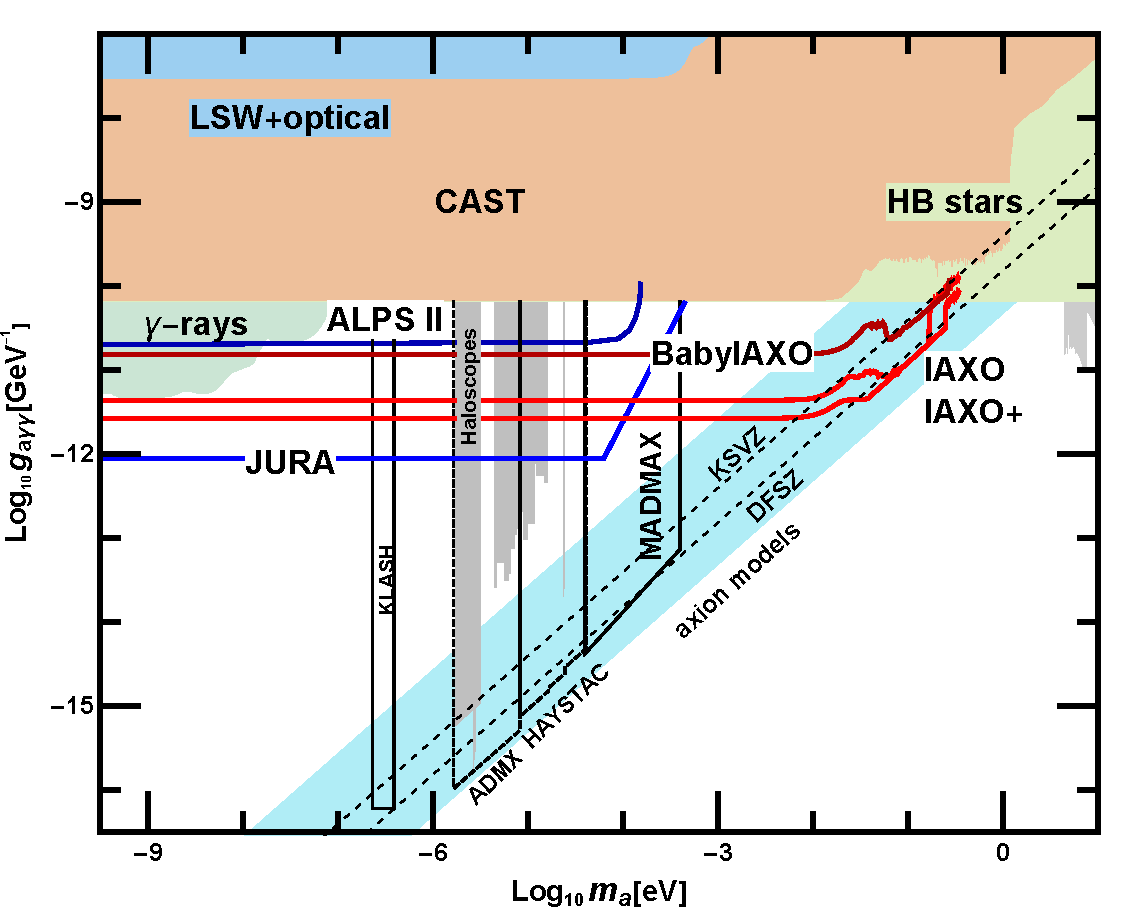
\includegraphics[width=0.7\textwidth]{Darkmatter/section4/esppalp2035.pdf}
\hspace*{1cm}
\caption{{Current exclusion of ALPs and axions coupling to photons in the sub-eV
mass-scale (see, e.g.,~\cite{Jaeckel:2010ni,Irastorza:2018dyq} for details) with experimental prospects. Astrophysical limits are shown in green, pure laboratory experiments are indicated in blue, helioscopes in red and haloscopes in black. The turquoise shaded region indicates the typical coupling range expected for QCD axion models. Couplings to other particles than photons are discussed in the support note.} }
\label{fig:alpsfig}	
\end{figure}

%%% 112 %%%%

Depending on the source of the ALPs there are currently three main search strategies:
\begin{enumerate}
\item[(i)] Direct detection with haloscopes~\cite{Sikivie:1983ip}, searching for ALPs being the dark matter.
\item[(ii)] Detection with helioscopes of ALPs being produced inside the Sun~\cite{Sikivie:1983ip}.
\item[(iii)] Experiments that produce and detect ALPs in the laboratory and are therefore independent of astrophysical and cosmological assumptions.
\end{enumerate}
%%%%
Current bounds on axions and ALPs and the reach of future experiments is shown
in Fig.~\ref{fig:alpsfig}.
Many of these experiments have overlap in technological requirements. The overlap in technologies, details of the below mentioned experiments and their synergies
are reviewed in~\cite{Siemko:2652165}.

\noindent{\bf (i) Haloscopes}: Amongst the axion haloscopes the US-led ADMX
%~\cite{Du:2018uak} 
and HAYSTAC
%~\cite{Zhong:2018rsr} 
experiments are at the forefront.
%, being the only running haloscope.
%{that published QCD-axion exlusions}, besides HAYSTAC.
ADMX is based on a resonant cavity approach, where axions are converted into photons via a magnetic field inside a
{radio-frequency} cavity. It {has started to} scan the lower mass part of the parameter space for the QCD axion. To go beyond the range explored by ADMX new geometries and technologies are being explored. In particular in Europe there are important developments with QUAX-a$\gamma$, %\cite{Alesini:2019ajt}
RADES, CAST-CAPP,
%\cite{Melcon:2018dba}
KLASH, %\cite{Gatti:2018ojx}
BRASS and CNRS/LNCMI-Grenoble.
%~\cite{Siemko:2652165}

At higher masses/frequencies, suggested in particular also by the post-inflationary axion scenario, a novel technique based on semi-resonant dielectric mirrors seems promising. The effort is named MadMax \cite{Majorovits:2017ppy} and is currently led by a collaboration between the MPI for Physics in Munich and DESY in Hamburg. 
The full scale version, that could reach axion sensitivity for a large fraction of the higher mass region is in preparation. 
%The costs are estimated to be around 20 million Euro. 

%In addition to these efforts that are mostly based on the coupling of axions to photons a number of proposals have been put forward to exploit other couplings, such as the defining one to gluons, but also to electrons. Experiments include Casper, QUAX and HeXenia that should develop on a short time-scale.
%We note that to fully establish the QCD axion nature and to reveal information on the underlying model it is necessary to probe the gluon and other couplings.
%\bigskip

\noindent {\bf (ii) Helioscopes:} Axion helioscopes aim to detect axions produced in the sun via photon-axion conversion. The signal is X-ray photons resulting from a 
re-conversion of axions into photons inside a strong magnet pointed at the sun. Importantly this signal is independent of axions being the dark matter. 
Building on the experience of the CAST experiment at CERN, that currently provides the best limits on the axion-photon coupling for sub-meV masses, IAXO aims at improving the sensitivity towards smaller couplings by about two orders of magnitude. This will provide a significant sensitivity to meV QCD axions as well as to ALPs that are plausible explanations of several astrophysical anomalies. Moreover, IAXO can also yield additional information beyond the photon coupling. It could deliver crucial information on axion-electron couplings as well as their mass. The IAXO physics potential has recently been summarized in~\cite{Armengaud:2019uso}.
IAXO received crucial support from CERN in the area of magnet design. A possible siting at DESY has been discussed.
A smaller-sized version dubbed BabyIAXO is ready to be built and could deliver physics results within less than 5 
years. 
%at a cost of about 5 million Euro. The full scale IAXO will benefit from this experience, {and} could be built directly after the first tests with BabyIAXO at an estimated cost of about 50 million Euro.

%\bigskip
\noindent {\bf (iii) Pure Laboratory Experiments:} Currently ALPS-II \cite{Bahre:2013ywa} is exploiting the light-shining-through-walls (LSW) technique where laser photons are converted to axions and back to photons inside strong magnetic fields. For masses below about $0.1\,{\rm meV}$ it aims to exceed the CAST sensitivity by about one order of magnitude in the coming years. It could thereby provide a robust test of the suggested astrophysical anomalies.
Using magnets planned  for a future collider, a large scale LSW experiment (JURA) could exceed the sensitivity of IAXO  in the low mass region by a factor of 3
or more in the future.
A ${\rm THz}$ photon source is proposed to be used in STAX (under R\&D now), instead of laser light,
profiting from a large photon number
%Huge photon number can be used with ${\rm THz}$ photon source. 

A different approach using Vacuum Magnetic Birefringence experiments has been proposed.
%When the strong magnetic field is applied 
%on the vacuum, the virtual electrons in the vacuum make
%Birefringence. 
%This is an effect of strong QED, but also
Their sensitivity for ALPs is, however, typically much smaller than LSW.
Running experiments based on this method are PVLAS and BMV, while in addition VMB@CERN has been proposed as new experiment. See e.g.~\cite{Siemko:2652165} for a detailed discussion.

\subsection{Complementarity with direct and indirect detection searches}
%\CW{JM: this moved here from section 1,  similar to the new 3.4, as discussed yesterday}
Radio searches for the conversion of axion/ALP dark matter into photons inside the magnetosphere of neutron stars can have sensitivity
%~\cite{Pshirkov:2007st,Huang:2018lxq,Hook:2018iia} 
for ALP masses in the range $\sim 0.2$--$40\,\mu$eV, and potentially above.  The signature is the emission of a narrow radio line from individual neutron stars, with a frequency that corresponds to the mass of the ALP.  Several of such searches are now underway, with expected sensitivities to the photon-ALP coupling down to $g_{a\gamma\gamma} \sim 10^{-12}\,\text{GeV}^{-1}$. The future SKA may have the ability to probe significant parts of the QCD axion parameter space.
%~\cite{Safdi:2018oeu}
 

Direct detection searches have sensitivity to ALP dark matter in the 1--100 keV mass region, via searches for an absorption triggered by the ALP-electron coupling. The currently best sensitivity is obtained by Xe detectors, which constrain the coupling of new pseudoscalars $g_{Ae} < 4 \times 10^{-13}$ in the 40--120 keV range.
%~\cite{Abe:2018owy}
Mid-term future experiments project a factor of $\sim$\,20 improvement.
%~\cite{Aalbers:2016jon}

%Similarly, with electron final states direct detection searches can constrain the kinetic mixing of vector particles. The leading constraints on vector bosonic dark matter coupling in the 0.1-10 keV/c$^2$ mass range come from Ge detectors~\cite{Singh:2018myp,Armengaud:2018cuy}.


\bigskip

% Move to Chap.5 by Shoji
%\subsection{Conclusions}
%The search for low energy particles like the axion has gained significant momentum. 
%{since the last ESPP \ref{lastinput}}
%Several experiments will explore promising regions in parameter space in the next ten years.
%Europe has unique opportunities to {take leadership} in %this worldwide effort.

%At a cost of about 50 million Euro 
%IAXO is a significant investment but provides the best opportunity to discover axions in the
%meV-eV mass range. 
%MadMax aims at the direct detection of axion dark matter in the $40-400\mu{\rm eV}$ mass range.
%with an estimated cost of about 20 million Euro is not yet fully strategic in scale but will benefit
%from efficient collaboration between large labs and universities.
%To exploit the innovative small scale efforts {and R\&D} that could {aid} the future discovery as well as high precision experiments,
%reliable support as well as collaboration with labs on key technologies is needed.

%\bibliography{/bib/section.bib}{}
%\bibliographystyle{report}


\end{document}

